\chapter{Contributions}
\label{sec:contributions}
%\fixme{(Figure: Fields in which we need instant feedback on appearance: 3d printing, artist feedback, quality control, meat)}
In this section, after introducing relevant theory and related work, we finally discuss the different contributions crated over the course of the Ph.D. studies. The goal of this section is to discuss the individual contributions in the light of the thesis goal. We remand to the text of the individual publications in Appendices~\ref{sec:firstcontribution}-\ref{sec:lastcontribution} for the full details.

From our discussion in Section~\ref{sec:motivation} we argue that there is a need in the industry for photorealistic accurate interactive rendering, i.e. the top-left area of Figure~\ref{fig:main_diagram}. In many fields, people need immediate feedback on on the aspect of the final product. Some examples include visual inspection of produced parts, preview of 3D printed objects, artistic iterations for movie scenes, and prediction of the outcomes of an industrial process. We showed in Figure~\ref{fig:main_results} where our contributions lie within the accuracy-time spectrum, addressing different accuracy and time targets depending on the application.

In this chapter, we will start by discussing the importance and the role of interactive photorealistic rendering presenting Contributions~\ref{sec:juice} and~\ref{sec:glass}. In the former, we make a case on why we need both fast and accurate rendering, in the form predicting the final appearance of cloudy apple juice from production parameters. In the latter Contribution~\ref{sec:glass}, we discuss how fast photorealistic rendering can be used for achieve accurate parameter estimation. We will then start diving into the interactive techniques we contributed with. In Contribution~\ref{sec:interactivedirsss} we discuss an interactive method to render with the directional BSSRDF described in Section~\ref{sec:analyticalbssrdf}. We will continue with Contribution~\ref{sec:srt}, a caching and filtering technique leveraging interactive ray tracing to improve temporal stability of rendered images. Moving forward, we will describe in Contribution~\ref{sec:vrbrdf} an application of physically based rendering in a virtual reality environment. Finally, we will conclude by discussing some future direction we could expand our work.

\section{Photorealistic rendering for appearance prediction and parameter estimation}
\label{sec:definingphoto}
\begin{figure}[t]
\centering
\begin{tabular}{@{}c@{}c@{}}
	 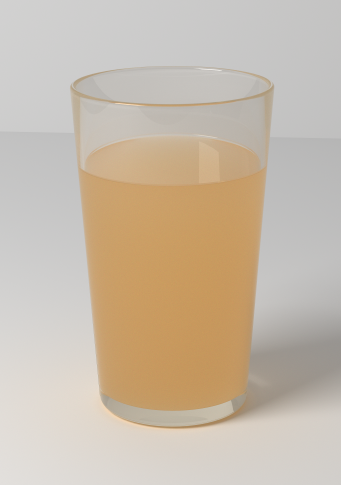
\includegraphics[width=0.4\columnwidth]{figures/teaser_render.png} &
	 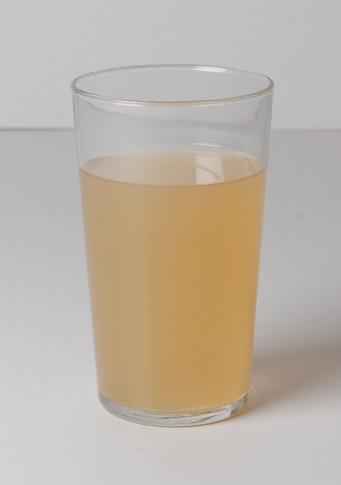
\includegraphics[width=0.4\columnwidth]{figures/ref_img.jpg}  \\
	rendering & photograph \\
\end{tabular}
\caption{Cloudy apple juice photographed and rendered the appearance model from Contribution~\ref{sec:juice}. In the model, we inferred apple particle concentration (0.8 g/l) and apple storage period (4 days) to match the photograph.} %The red rectangle shows where we estimated RMSE in Table \ref{table:quant}.}
\label{fig:juicecomparison}
\end{figure}

We start our discussion from Contributions~\ref{sec:juice} and \ref{sec:glass}. Our first discussion point is about validating physically based rendering. In literature, the emphasis is often onto creating rendering models and techniques that effectively approximate an arbitrary radiometric process. However, not much emphasis is put into validating the developed models with an image of a physical object, like we do in Figure~\ref{fig:juicecomparison} from Contribution~\ref{sec:juice}. In the figure, we compare two pictures of cloudy apple juice, one a picture of an actual glass of juice, one a rendering representation of it using interactive volumetric path tracing (12 samples per pixel per second), with the algorithm described in~\ref{sec:volumept}. In literature, authors usually rely on path traced references, like the one on the left of the figure, since it is much easier to compare to that than to an actual picture. Our first Contributions~\ref{sec:glass} and~\ref{sec:juice} originally were developed with the purpose to test the limits of physically based rendering, testing how close a rendering using path tracing can get to real images. Both investigations led to a number of interesting insights on physically based rendering.

\begin{figure}[t]
\centering
\begin{tabular}{@{}c@{}c@{}}
	 & Increasing concentration $\longrightarrow$ \\
	\begin{sideways}\hspace{1em}$\longleftarrow$ Days stored \end{sideways} \hspace{0.5mm} &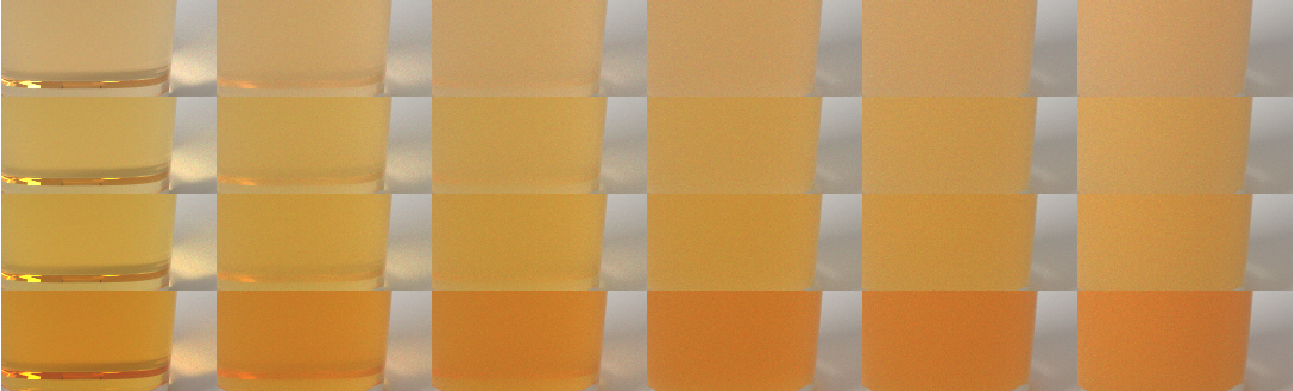
\includegraphics[width=0.9\columnwidth]{figures/comparison_renderings.png} \\
	 \begin{sideways}\hspace{1em}$\longleftarrow$ Days stored \end{sideways} \hspace{0.5mm} &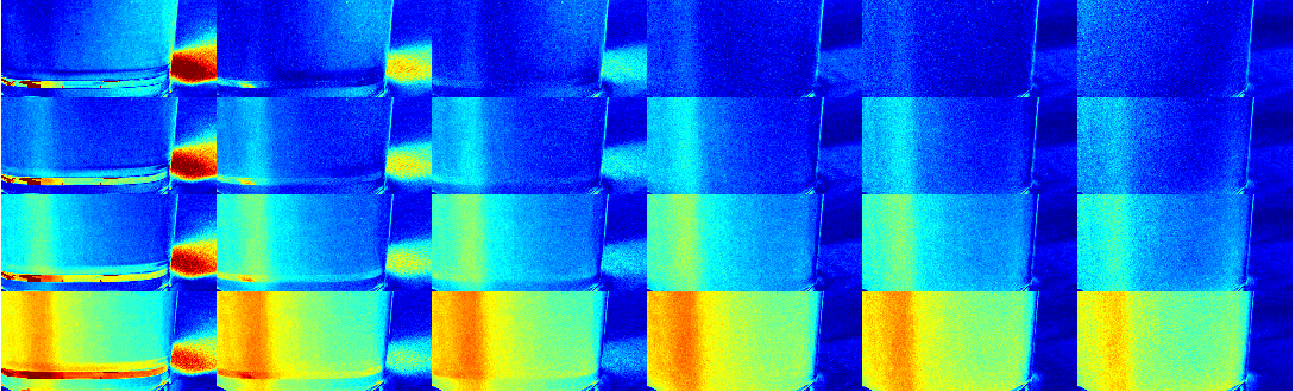
\includegraphics[width=0.9\columnwidth]{figures/comparison_diff.png}  \\
	 & Increasing concentration $\longrightarrow$

\end{tabular}
\caption{Comparing a patch of various renderings of cloudy apple juice in Contribution~\ref{sec:juice}. The horizontal axis shows increasing concentration, while the vertical axis shows the number of days the apples have been stored before pressing them. The top image shows the actual renderings, the bottom image shows false-color comparisons to reference (red is higher error).}
\label{fig:juicecomparisondetail}
\end{figure}

In our first Contribution~\ref{sec:juice}, we created a combined appearance model to predict the appearance of cloudy apple juice. The goal here is to be able to predict the final appearance of apple juice by changing production parameters, such as the concentration of the juice or the type of environment the apples are pressed. The business case would be for a juice company to predict appearance changes due to a change in the concentration of apples in the juice, with the constraint that the final product is still should still be appeasing for the customer. Given that the space of production parameters is potentially huge, it is important to give immediate feedback using accurate physically based rendering so that various possible parameter configurations can be tested quickly. This comparison framework could be used in both directions: as prediction for the final appearance, but also to measure the production parameters of an unknown sample. 

A first insight is that if the scene is carefully set and calibrated, a comparison is definitely possible, and actual production parameters can be estimated. We can see this in Figure~\ref{fig:juicecomparisondetail}, where we compare a patch of the final rendering result with reference. We observed the biggest issue to be in carefully setting and calibrating the scene. In this first proof of concept, we placed the objects and the light in the rendered scene manually, using reasonable estimates for their geometry and appearance parameters. This contribution led to discover a number of different challenges in comparing pictures and renderings, mostly related to the scene. Subtle changes in the scene lead to big differences in direct comparisons, especially when the material influences its surroundings, such and in the case of cloudy apple juice. See the light caustic next to the glass in Figure~\ref{fig:juicecomparisondetail}. In this initial proof of concept, we simply compared a patch to get a reasonable parameter estimate. In the next Contribution~\ref{sec:glass}, we set into improving the whole process of comparison and data reconstruction.

\begin{figure}
\centering
 \includegraphics[width=0.8\textwidth]{figures/comparison} 
\caption{Comparing quantitatively renderings (top row) with real images (mid row). Log-error is shown on the bottom row.}
\label{fig:glasscomparison}
\end{figure}

\begin{figure}
\centering
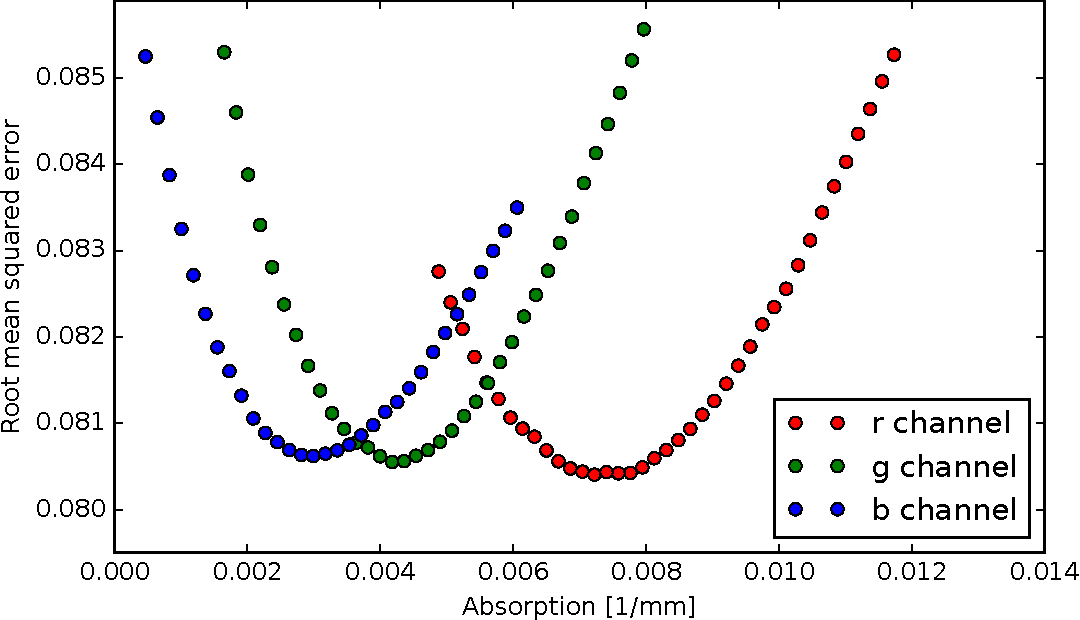
\includegraphics[width=0.9\textwidth]{figures/glass_bowl_analysis_by_synthesis}  \caption{Estimating the absorption parameter $\sigma_a$ for the glass bowl in Figure~\ref{fig:glasscomparison}. Each coefficient was estimated independently. Each dot in the graph corresponds to a rendered image. }
\label{fig:glasscomparisongraph}
\end{figure}

Our proof of concept in Contribution~\ref{sec:juice} is dual. First, it tells us that it is important to validate renderings with photographs, to ensure that the rendering matches the appearance in the real world. Secondly, it tells us that to have multiple parameters tested or estimated, depending on the application, we need fast rendering. We discuss the first aspect in the rest of this section, referring to the next section for a more complete discussion on fast rendering of scattering materials. In our Contribution~\ref{sec:glass}, we strive to improve upon the previous results of comparing rendering with images, for a slightly different application. In this case, we are comparing images of glass objects. As it is true for scattering materials, the appearance of glass objects (see Section~\ref{sec:glassdescr}) is greatly influenced by the surrounding scene, making the scene estimation arguably even more important for this application. We use a full pipeline to accurately estimate the scene, scan glass objects with CT scanners and place them in the scene for final rendering. Our main contribution of this work is actually the pipeline, that allows researchers to compare pictures and renderings of glass objects, getting a quantitative comparison at the end. Some results are in Figure~\ref{fig:glasscomparison}. This ability of qualitatively compare images and rendering allows to further improve existing techniques in acquisition, rendering and reconstruction. As another goal of our improved reconstruction results, we can estimate material properties much more accurately than our  results in Contribution~\ref{sec:juice} and in Figure~\ref{fig:juicecomparisondetail}. We measure both the relative index of refraction $\eta$ and the spectral absorption coefficient $\sigma_a$ for each of the glass objects, as we can see in Figure~\ref{fig:glasscomparisongraph}, where we show the results for the spectral components of the estiamted $\sigma_a$. Note that each point of the graph is a rendering, further proving the point to use fast rendering to generate a great number of images to estimate the material properties. Since we want accuracy, we need to use unbiased path tracing, that we accelerate using the GPU and execute at lower resolutions to achieve fast and accurate rendering of these images. In this particular case, our renderings are accurate enough for parameter estimation after a few minutes. 

\section{Interactive rendering of scattering media}
\label{sec:interactivedirssscontribution}
%
\begin{figure}[t]
\begin{tabular}{@{}c@{}c@{}c@{}c@{}}
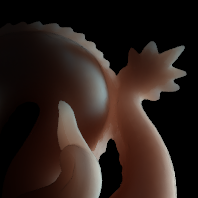
\includegraphics[width=0.27\columnwidth]{figures/difference/dragon_shampoo_jensen} &
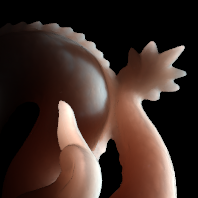
\includegraphics[width=0.27\columnwidth]{figures/difference/diff_dr_ours_small} &
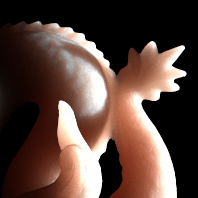
\includegraphics[width=0.27\columnwidth]{figures/difference/diff_dr_ref_small} &
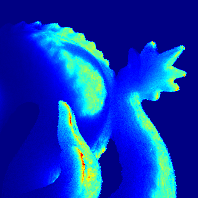
\includegraphics[width=0.27\columnwidth]{figures/difference/diff_dr_diff_small} \\ 
our method & our method & unbiased & difference  \\
\cite{Jensen2001} & \cite{Frisvad2014} & \cite{Frisvad2014} &  \\
\end{tabular}
\caption{Comparing our interactive rendering method, with different dipoles and against the unbiased rendering technique reported in Appendix~\ref{sec:pointcloudnote}.}
\label{fig:interactivediff}
\end{figure}
%
\begin{figure}[t]
\centering
\begin{tabular}{@{}c@{$\,$}c@{}c@{}c@{}}
& directional dipole, 6 fps & standard dipole and VPLs \\
\begin{sideways}\hspace*{1.5em}our method\end{sideways}\hspace{0.5mm} &
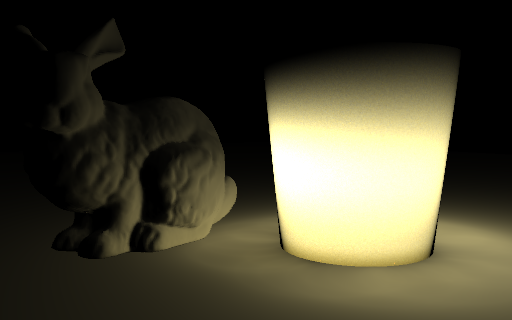
\includegraphics[width=0.43\columnwidth]{figures/candle_holder_directional_6fps.png} &
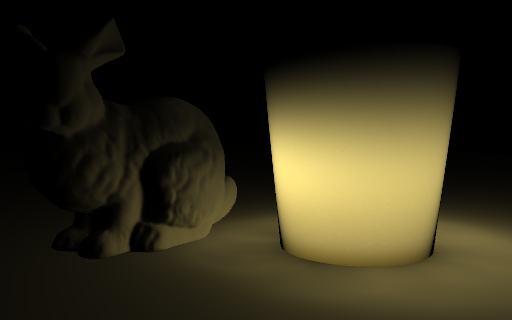
\includegraphics[width=0.43\columnwidth]{figures/candle_holder_jensen_converged.png} \\[-4pt]
\begin{sideways}\hspace*{1.7em}ray tracer\end{sideways}\hspace{0.5mm} &
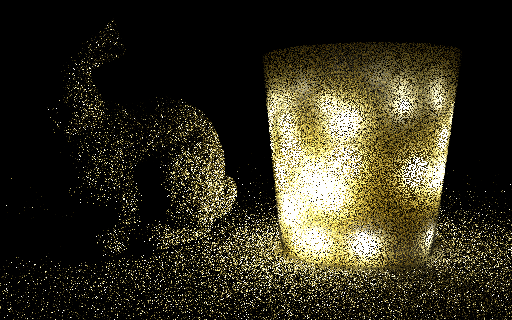
\includegraphics[width=0.43\columnwidth]{figures/scene_comparison_optix_6fps.png} &
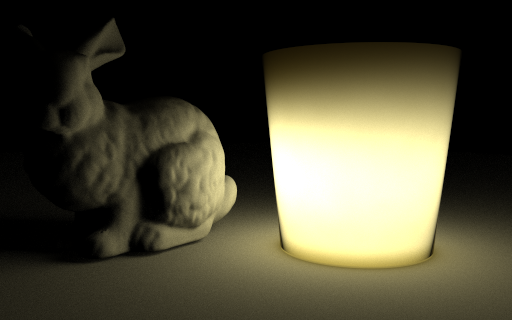
\includegraphics[width=0.43\columnwidth]{figures/scene_comparison_converged.png} \\[-0.5ex]
& directional dipole, 6 fps & directional dipole, reference \\[-1ex]
\end{tabular}
\caption{Equal time comparison (left column) of our method with the reference method and qualitative comparison with diffuse subsurface scattering (upper right) and the converged reference solution (Appendix~\ref{sec:pointcloudnote}, lower right). The scene is lit by a point light in a white grapefruit candle holder.} % Emerging light illuminates a diffuse Stanford Bunny on a tabletop.}
\label{fig:optixcomparison}
\end{figure}
%
After discussing photorealistic rendering in the previous section, in this section we start discussing our first interactive technique. We also here take inspiration from Contribution~\ref{sec:juice}: in the previous section, we discussed the importance of physically based rendering for material prediction and acquisition. In this section, we acknowledge the fact that for many applications, including previews, games, etc. we can accept lower accuracy in our renderings (see Figure~\ref{fig:main_results}). In this technique, we achieve a photorealistic look using the BSSRDF approximation presented in Section~\ref{sec:bssrdfgeneral}.

Our Contribution~\ref{sec:interactivedirsss} is a rasterization-based caching scheme to improve photorealism of existing techniques. The most important contribution in this technique is that allows rendering using \emph{directional} BSSRDFs, like the directional dipole discussed in Section~\ref{sec:analyticalbssrdf}. In particular, our technique allows to render with any BSSRDF analytical model that depends on $\vec{\omega}_i$, the direction of the incoming light. In Figure~\ref{fig:interactivediff} we can see a  comparison between the standard dipole~\cite{Jensen2001} and the directional dipole~\cite{Frisvad2014} in the first two images. The directional dipole allows more subtle scattering effects to be computed, accounting partially for single scattering, that in previous techniques needed to be added separately. Unfortunately, most of the interactive and real time techniques for rendering BSSRDFs assume that the BSSRDF is function of the distance $r$ between the point of incidence and emergence. This can be exploited for different optimizations, like filtering, precomputation or tabulation, that are not feasible anymore when it comes to using a directional technique. Our technique is unique in handling this specific type of directional dipoles in the interactive domain. 

In the classification of different techniques presented in Chapter~\ref{sec:related}, our technique is mostly a caching technique, with some filtering required to assemble the final image. Our technique leverages the strengths of rasterization, storing progressive maps of scattered radiosity rendered from different directions around the object. We can now account for the directionality of the light in the computation, and in addition progressively store the intermediate result as soon as the light and the object do not change. The technique is not real time but interactive (80 to 160 milliseconds on a 2014 GPU), and does not require neither precomputation nor texture parameterization. Given this features, we can apply this technique to procedural deformable objects, something that is generally difficult to achieve with precomputation techniques. We also proposed an improved sampling scheme, that via a light G-buffer samples always close to the light source, allowing light to propagate through objects and around sharp corners. This can be seen in particular in Figure~\ref{fig:optixcomparison}, in the top left image, where a point light source is places inside a candleholder made of a scattering material. Figure~\ref{fig:interactivediff} shows the price we pay for our improved technique, since it introduces some artifacts in the rendering of the directional dipole, visible as dimming. We can see this comparing and showing the difference against the ray tracing based unbiased rendering technique for scattering materials reported in Appendix~\ref{sec:pointcloudnote}.

As another contribution of our technique, we leverage our scattered radiosity maps to place VPLs on the surface of the objects. This allows to transfer emergent light onto other surfaces. An example can be seen in Figure~\ref{fig:optixcomparison}, where we transport the light from a point light inside an object on the outside, illuminating the bunny on the tabletop. In the same figure, we can see on how we successfully compare to the technique in Appendix~\ref{sec:pointcloudnote}, that in the same time cannot achieve the same results, looking non converged and noisy (bottom left).

To sum up, the take away home message of this technique is that improved physical models, such as the directional dipole, sometimes do not allow us to reuse previous work. So, we need to develop new techniques to achieve interactive result, so that we can include these more accurate effects. Moreover, the benefits of caching data in this case become particularly apparent, since they allow us to recycle the stored radiosity for another technique to use. 

\section{Interactive stable ray tracing}
\label{sec:srtcontribution}
\begin{figure}[t]
\begin{tabular}{@{}c@{}c@{}@{}c@{}}
	 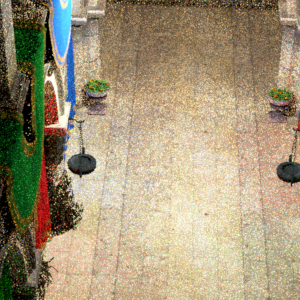
\includegraphics[width=0.32\textwidth]{figures/ss_2x_rect_370_300_300_300_frame_211.png} &
		 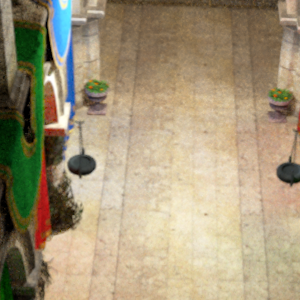
\includegraphics[width=0.32\textwidth]{figures/ss_2x_taa_rect_370_300_300_300_frame_211.png} &
		  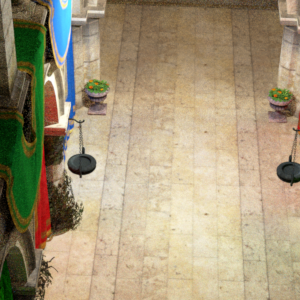
\includegraphics[width=0.32\textwidth]{figures/ss_32x_rect_370_300_300_300_frame_211.png} \\	 
Supersampling, 2 spp & Supersampling, 2 spp 	& Supersampling, 32 spp \\
  					 & + temporal antialiasing 	&  \\
sharpness: 0.7924 & sharpness: 0.5348 & sharpness: 0.6771  \\
	 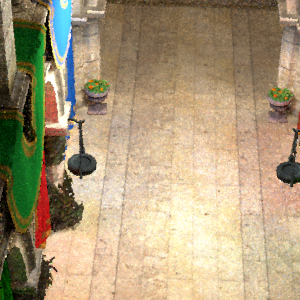
\includegraphics[width=0.32\textwidth]{figures/srt_1_rect_370_300_300_300_frame_211.png} &
	 	 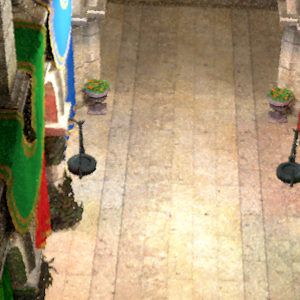
\includegraphics[width=0.32\textwidth]{figures/srt_1_ti_rect_370_300_300_300_frame_211.png} &
	  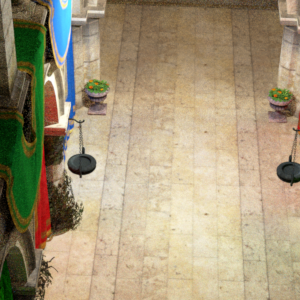
\includegraphics[width=0.32\textwidth]{figures/ss_32x_rect_370_300_300_300_frame_211.png}
 \\
Stable RT, 1 spp & Stable RT, 1 spp & Supersampling, 32 spp \\
 & + temporal integration &  \\
sharpness: 0.7085 & sharpness: 0.6060 & sharpness: 0.6771 \\[-1.5ex]
\end{tabular}
\caption{Different techniques applied to a frame in the Sponza video, equal time comparison. Sharpness is also shown (higher is sharper). Stable ray tracing offers a less noisy result (first column) compared to reference (third column). When temporal techniques are applied (second column) Stable ray tracing yields the sharper result.  }
\label{fig:sponza_video_frame}
\end{figure}

After dealing with subsurface scattering, we continue exploring the spectrum of interactive photorealistic techniques in stable ray tracing, Contribution~\ref{sec:srt}. As in the previous section, we use caching as a technique to improve existing physically based techniques. In the previous section, we created a technique that anchors the scattering contribution to the surface of the object using depth-augmented scattered radiosity maps. In stable ray tracing, we solve a completely different problem, but that in the essence has the same overall purpose, caching points on surfaces. In this contribution, in particular, we track these points in order to achieve temporally stable renderings. 

Our technique was developed with interactive ray tracing in mind. In interactive or real time ray tracing, the number of rays we can trace per pixel becomes extremely limited, in the order or one or two full paths. Also, the shading locations change every frame, causing a noisy image, both spatially and temporally. Existing techniques, namely temporal anti aliasing~\cite{Karis2014}, can mitigate the problem, though they generally introduce blurring. In our technique, we recycle shading locations across frames using a screen space data structure. By shading always the same points, we improve temporal stability, while retaining sharpness as well. We achieve this at interactive frame rates (20-60 milliseconds per frame). We can see the results in Figure~\ref{fig:sponza_video_frame}. In the result we can see how stable ray tracing yields a sharper result than temporal antialiasing. The technique contributes as a rendering system to improve temporal stability: other existing techniques can be further applies on top to further improve shading quality. 

Another contribution of this technique is that it shows how we can leverage the strength of one interactive technique, namely ray tracing, against the most commonly used rasterization. Current hardware does not allow shading locations to be arbitrarily chosen within a pixel, relying on fixed patterns. In our technique, we allow shading locations to vary in screen space per pixel, while staying the same in world space. 

Finally, another advantage of this technique, in particular in a photorealistic rendering context, is that it allows to store information across frames. In the paper, we present an example case where we store indirect path traced illumination. This will allow in the future to extend the technique with other sort of data, to further improve the technique. This gives the take home message of this technique: we need generic, robust techniques that can be applied in a variety of situations, inexpensive and that can work together with existing techniques. We believe that stable ray tracing satisfies these characteristics. 

A particular application where the stable ray tracing caching scheme would be particularly useful is virtual reality. Because of the close vicinity of the eye to the display and the perception system in our eyes, temporal stability issues are particularly obvious. Unfortunately, given the real time requirements for virtual reality this technique is not applicable at the moment.

\section{Applying interactive photorealistic techniques}
\label{sec:vrbrfcontribution}
\begin{figure}[t]
\centering
\begin{tabular}{@{}c@{}c@{}}
	 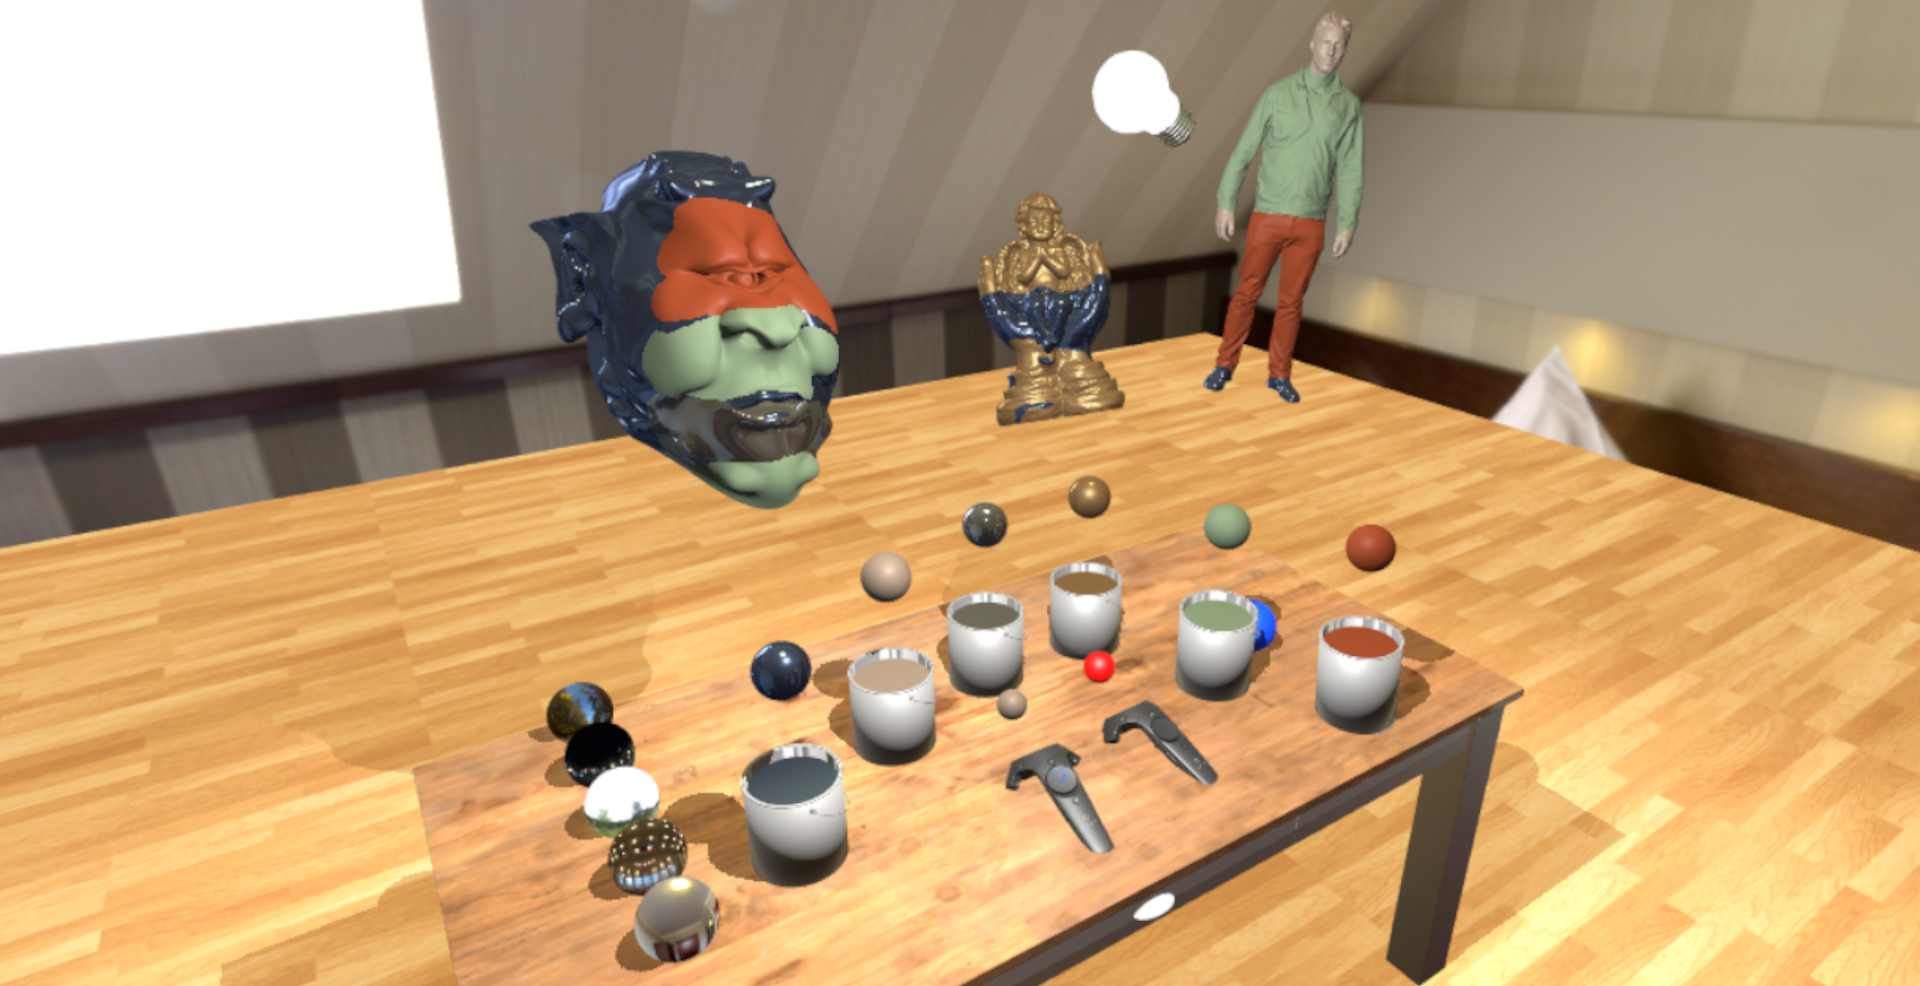
\includegraphics[height = 4.3cm]{figures/screen1_crop} &
		 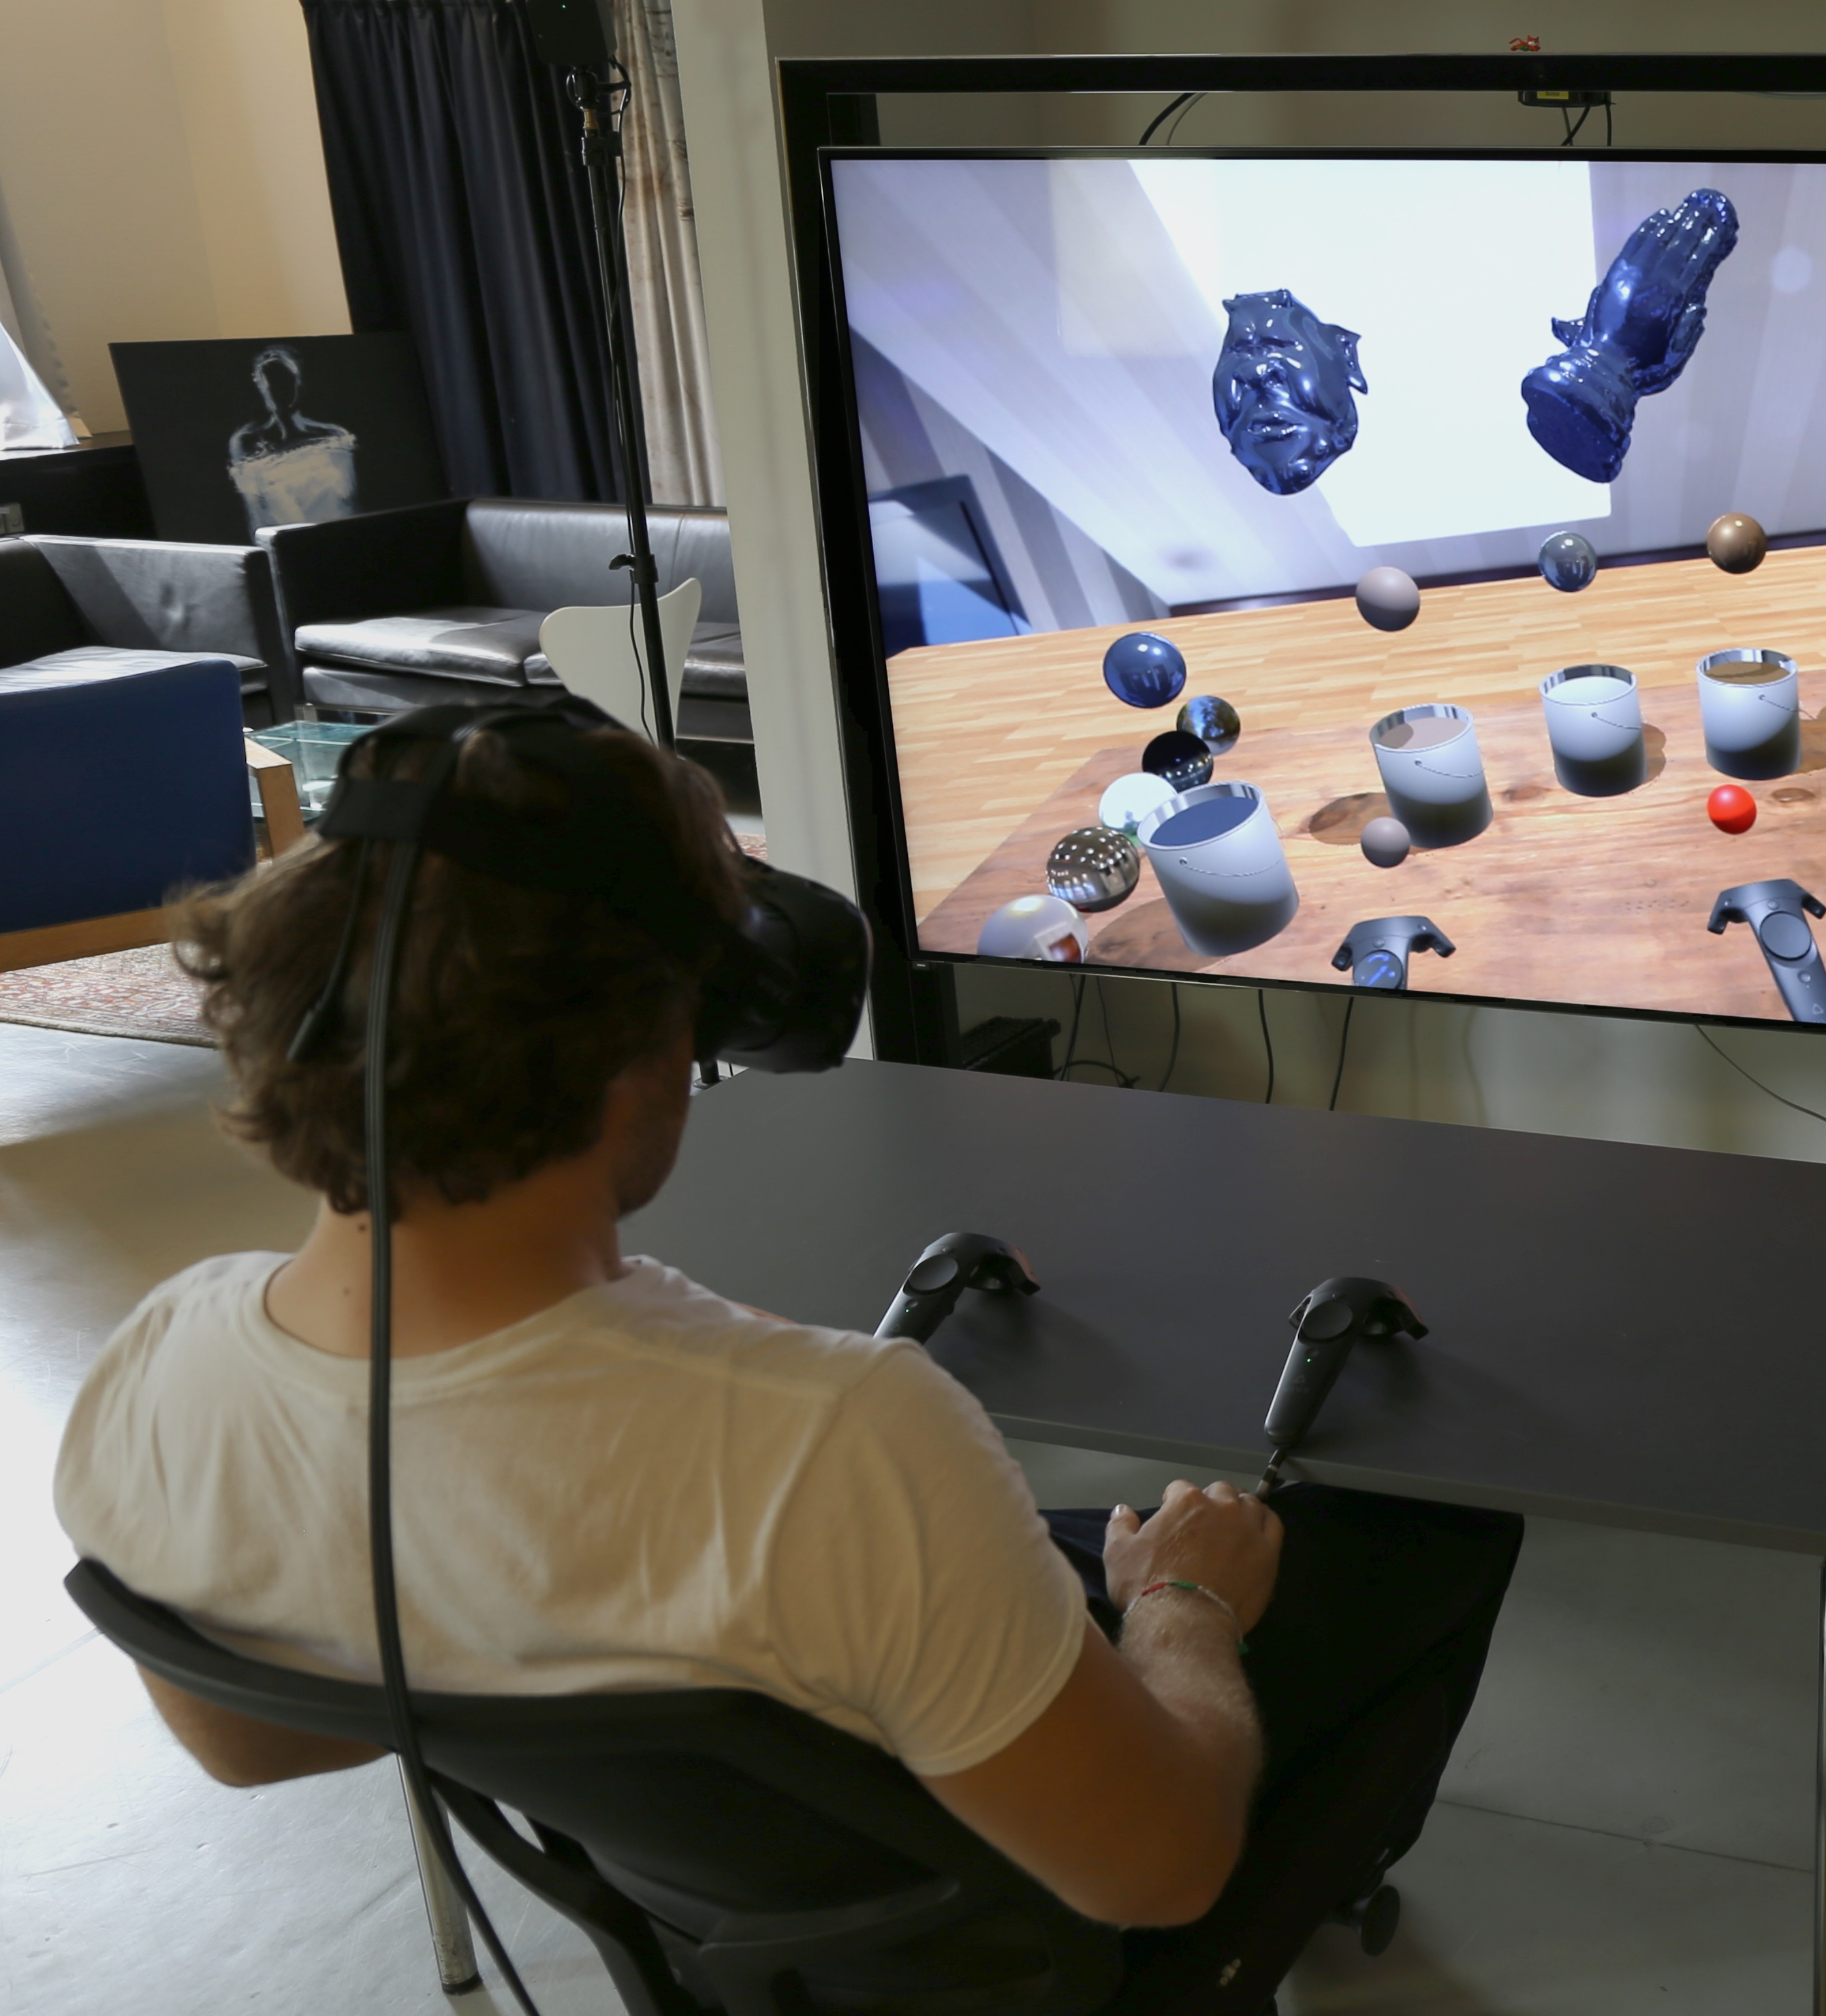
\includegraphics[height = 4.3cm]{figures/person} \\[-2.5ex]
\end{tabular}
  \caption{Pictures illustrating our VR demo application, with an in-game screenshot (left) and a picture of the setup (right). }
  \label{fig:vrbrdfimage}
\end{figure}
In the final paper we discuss in Contribution~\ref{sec:vrbrdf}, we discuss a proof of concept for virtual reality rendering of physically based materials. In this context, applications need to consistently perform at 90 frames per second or faster, to avoid issues for the users, e.g. dizziness or motion sickness. In our application, we modify the rendering pipeline of the Unity game engine to include measured BRDFs, in the discretized form of the MERL database, as described in Section~\ref{sec:empiricalbrdf}. The application provides a painting environment for artists to paint on object surfaces using measured BRDFs, using a HTC Vive headset and controllers. The environment includes the possibility to move and rotate objects, paint with different sized brushes, a movable light and a undo button. The direct illumination is given by a point light, plus low frequency environment illumination using spherical harmonics. A reflection map is added on top, with intensity depending on the specularity of the material, and depending on the ratio between peak and average value of the BRDF. The overall simulation renders at steady 11 milliseconds per frame.

This proof of concept was born as an inspecting tool to debug physically based materials, aided by the provided in-game controllers (see an example image in Figure~\ref{fig:vrbrdfimage}). The application shows once more how important is to achieve interactive photorealistic rendering in virtual reality, giving a glimpse on how photorealistic materials are able to augment the immersiveness of the application. 

\section{Discussion}
In the previous sections, we showed how our contribution overall contribute to the goal of expanding interactive technique towards a more physically accurate framework. The natural step of the topics discussed in this thesis is to further expand the techniques in photorealism, by including as an example more accurate physical models, but retaining the same performance level. In the following, we discuss some possible avenues of expansion of our work.

\textbf{Validating path tracing}. Some avenues are possible in continuing the work we initiated in Contributions~\ref{sec:juice} and \ref{sec:glass}. In particular, we would like to continue our initial goal of validating path tracing. This would require expanding the technique to be more accurate, in particular in regards to geometry. For a more complete validation, we would like to expand the technique to handle fully scattering materials instead of glass only. Other avenues of research are possible in regards of estimating parameters: scattering parameters ($\sigma_a$, $\sigma_s$ and $g$) are obvious candidates for a further expansion.

\textbf{Hybrid rasterization-ray tracing rendering techniques}. As for now, we focused on our technique to be exclusively rasterization or ray tracing based. Some potential improvements can be thought by combining the two techniques. For example, some could think of an extension of our stable ray tracing in Contribution~\ref{sec:srt} to support our technique from Contribution~\ref{sec:interactivedirsss}. In this particular case, the scattered radiosity maps can be replaced by the stable ray traced points. The rasterization of the light G-buffer would still have to be executed, making this an hybrid technique.  Another example, in our virtual reality contribution~\ref{sec:vrbrdf}, would be to evaluate reflections via ray tracing, to properly include the overall contribution instead of an approximation via a precomputed probe.

\textbf{Virtual reality}. In recent year, virtual reality has become more prominent in real time applications. Given the hard constraints of virtual reality, the techniques we developed would need to be adapted to fit a virtual reality environment. In particular our stable ray tracing algorithm in Contribution~\ref{sec:srt} seems like a good fit for a virtual reality environment, that is particularly plagued by temporal stability issues. 

\textbf{Dataset generation for machine learning}. Interactive techniques for photorealistic rendering allow generating image data much faster than traditional techniques. This makes them particularly useful to generate synthetic data to train image based machine learning techniques.  